\documentclass[a4paper,UTF8]{article}
\usepackage{ctex}
\usepackage[margin=1.25in]{geometry}
\usepackage{color}
\usepackage{graphicx}
\usepackage{amssymb}
\usepackage{amsmath}
\usepackage{amsthm}
\usepackage{soul, color, xcolor}
\usepackage{bm}
\usepackage{tcolorbox}
\usepackage{hyperref}
\numberwithin{equation}{section}
%\usepackage[thmmarks, amsmath, thref]{ntheorem}
\theoremstyle{definition}
\newtheorem*{solution}{Solution}
\newtheorem*{prove}{Proof}
\DeclareMathOperator{\diag}{diag}
\usepackage{multirow}
\usepackage{diagbox}
\usepackage{float}

\setlength{\parindent}{0pt}
\newcommand{\bds}{\boldsymbol}
\def \X {\mathbf{X}}
\def \A {\mathbf{A}}
\def \C {\mathbf{C}}
\def \w {\hat{\boldsymbol{w}}}
\def \y {\mathbf{y}}
\def \x {\mathbf{x}}
\def \z {\mathbf{z}}
\def \hy {\widehat{y}}
\def \by {\Bar{y}}
\def \H {\mathbf{H}}
\def \I {\mathbf{I}}
\newcommand\given[1][]{\:#1\vert\:}


\begin{document}
\title{机器学习导论\ 习题二}
\author{211300044, 吴羽珩, \href{mailto:邮箱}{2559280859@qq.com}}
\maketitle
\section*{作业提交注意事项}
\begin{tcolorbox}
	\begin{enumerate}
		\item[1.] 请在LaTeX模板中第一页填写个人的学号、姓名、邮箱;
		\item[2.] 本次作业需提交作答后的该 pdf 文件、编程题~.ipynb 文件; {\color{red}\textbf{请将二者打包为~.zip 文件上传}}. 注意命名规则, 三个文件均命名为 “$\text{学号}\_\text{姓名}$” + “.后缀” (例如 $\text{211300001}\_\text{张三}$” + “.pdf”、“.ipynb”、“.zip”);
		\item[3.] 若多次提交作业, 则在命名~.zip 文件时加上版本号, 例如 211300001\_张三\_v1.zip” (批改时以版本号最高的文件为准);
		\item[4.] 本次作业提交截止时间为 {\color{red}\textbf{ 4 月 19 日23:59:59}}. 未按照要求提交作业, 提交作业格式不正确, {\color{red}\textbf{作业命名不规范}}, 将会被扣除部分作业分数; 除特殊原因 (如因病缓交, 需出示医院假条) 逾期未交作业, 本次作业记 0 分; {\color{red}\textbf{如发现抄袭, 抄袭和被抄袭双方成绩全部取消}};
		\item[5.] 本次作业提交地址为 \href{https://box.nju.edu.cn/u/d/72f6f8cfff054611b6d3/}{here}, 请大家预留时间提前上交, 以防在临近截止日期时, 因网络等原因无法按时提交作业.
	\end{enumerate}
\end{tcolorbox}
\newpage


\section{[20pts] Linear Discriminant Analysis}
线性判别分析 (Linear Discriminant Analysis, 简称 LDA) 是一种经典的线性学习方法. 请仔细阅读《机器学习》第三章 3.4 节, 并回答如下问题.

\begin{enumerate}
	\item[(1)] \textbf{[10pts]} (二分类) 假设有两类数据, 其中正类服从高斯分布$P=\mathcal{N}\left(\bds{\mu}_1, \bds{\Sigma}_1\right)$, 负类服从高斯分布 $Q=\mathcal{N}\left(\bds{\mu}_2, \bds{\Sigma}_2\right)$. 对于任一样本 $\bds{x}$, 若分类器 $h$ 满足:
     $$
     h(\bds{x})= \begin{cases}0 & P(\bds{x})\leq Q(\bds{x}), \\ 1 & P(\bds{x})>Q(\bds{x}), \end{cases}
     $$
     则认为 $h$ 实现了最优分类. 假设 $\bds{\mu}_1,\bds{\mu}_2, \bds{\Sigma}_1, \bds{\Sigma}_2$ 均已知, 请证明当 $\bds{\Sigma}_1=\bds{\Sigma}_2=\bds{\Sigma}$ 时, 通过 LDA 得到的分类器可实现最优分类.
     (提示: 找到满足最优分类性质的分类平面)
	\item[(2)] \textbf{[10pts]} (多分类) 将 LDA 推广至多分类任务时, 可采用教材中式 (3.44) 作为优化目标. 通过求解式 (3.44), 可得到投影矩阵 $\mathbf{W}\in \mathbb{R}^{d\times d'}$, 其中 $d$ 为数据原有的属性数. 假设当前任务共有 $N$ 个类别, 请证明 $d'\leq N-1$. (提示: 对于任意 $n$ 阶方阵, 其非零特征值个数小于等于其秩大小)
\end{enumerate}


\begin{solution}
	此处用于写解答 (中英文均可)
	\begin{itemize}
		\item[(1)] 当$\bds{\Sigma}_1=\bds{\Sigma}_2=\bds{\Sigma}$时 \\
		设最优平面为$\bds{a}^T\bds{x}=b$,由最优分类的性质,易知在最优分类平面上的点 $\bds{x}$,一定满足 $P(\bds{x}) = Q(\bds{x})$. 由此可得
		\begin{equation}
			\begin{split}
				c\cdot \bds{\Sigma}^{-\frac{1}{2}}e^{-\frac{1}{2}(\bds{x} - \bds{\mu}_1)^T\bds{\Sigma}^{-1}(\bds{x}-\bds{\mu}_1)} &= c\cdot \bds{\Sigma}^{-\frac{1}{2}}e^{-\frac{1}{2}(\bds{x} - \bds{\mu}_2)^T\bds{\Sigma}^{-1}(\bds{x}-\bds{\mu}_2)} \\
				-\frac{1}{2}(\bds{x} - \bds{\mu}_1)^T\bds{\Sigma}^{-1}(\bds{x}-\bds{\mu}_1) &= -\frac{1}{2}(\bds{x} - \bds{\mu}_2)^T\bds{\Sigma}^{-1}(\bds{x}-\bds{\mu}_2) \\
			\end{split}
			\notag
		\end{equation}
		整理得:
		$$
		\frac{1}{2}(\bds{\Sigma}^{-1}(\bds{\mu}_2-\bds{\mu}_1))^T \bds{x} = \frac{1}{4}(\bds{\mu}_2+\bds{\mu}_1)^T\bds{\Sigma}^{-1}(\bds{\mu}_2-\bds{\mu}_1) 
		$$
		即:\\$\bds{a}=\frac{1}{2}\bds{\Sigma}^{-1}(\bds{\mu}_2-\bds{\mu}_1)$\\
		$b=\frac{1}{4}(\bds{\mu}_2+\bds{\mu}_1)^T\bds{\Sigma}^{-1}(\bds{\mu}_2-\bds{\mu}_1)$\\
		根据LDA分类器的计算步骤,计算 $\bds{w}$,由教材公式(3.39)可得
		\begin{equation}
			\begin{split}
				\bds{w} &= \mathbf{S}_{w}^{-1}(\bds{\mu}_1-\bds{\mu}_2) \\
				&= (\bds{\Sigma}_1+\bds{\Sigma}_2)^{-1}(\bds{\mu}_1-\bds{\mu}_2) \\
				&= \frac{1}{2}\bds{\Sigma}^{-1}(\bds{\mu}_1-\bds{\mu}_2)\\
				&= \bds{a}
			\end{split}
			\notag
		\end{equation}
		我们发现$\bds{a}=\bds{w}$,进一步发现两类样本投影中心 $\bds{\mu}'_1 = \frac{1}{2}\bds{\mu}_1^T\bds{\Sigma}^{-1}(\bds{\mu}_1-\bds{\mu}_2), \quad \bds{\mu}'_2 = \frac{1}{2}\bds{\mu}_2^T\bds{\Sigma}^{-1}(\bds{\mu}_1-\bds{\mu}_2)$,其中点为
		\begin{equation}
			\begin{split}
				\bds{\mu}' &= \frac{1}{2}(\bds{\mu}'_1+\bds{\mu}'_2) \\
				&= \frac{1}{4}(\bds{\mu}_1+\bds{\mu}_2)^T\bds{\Sigma}^{-1}(\bds{\mu}_1-\bds{\mu}_2)\\
				&= b
			\end{split}
			\notag
		\end{equation}
		于是有由LDA得到的分类平面为
		\begin{equation}
			\begin{split}
				\bds{x}^T\bds{w} - \bds{\mu}' &= 0 \\
			\end{split}
			\notag
		\end{equation}
		所以在 $\bds{\Sigma_1} = \bds{\Sigma_2} = \bds{\Sigma}$时,通过LDA得到的分类器可实现最优分类.
		\item[(2)]
		矩阵 $$\textbf{S}_b = \sum_{i=1}^{N}m_i(\bds{\mu}_i-\bds{\mu})(\bds{\mu}_i-\bds{\mu})^T$$所以 $\textbf{S}_b$为$N$个 $m_i(\bds{\mu}_i-\bds{\mu})(\bds{\mu}_i-\bds{\mu})^T$的矩阵之和,对于$N$个矩阵中的任意一个矩阵$A_i$由于 $(\bds{\mu}_i-\bds{\mu})(\bds{\mu}_i-\bds{\mu})^T$的所有行向量均线性相关,所以 $$\text{Rank}(A_i)=\text{Rank}((\bds{\mu}_i-\bds{\mu})(\bds{\mu}_i-\bds{\mu})^T) = 1$$ 所以 $$\text{Rank}(\textbf{S}_b) \leq \sum_{i=1}^{N} \text{Rank}(A_i) = N$$ \\
		一共有 $N$个类别,当我们得到 $N-1$个类别的均值 $\bds{\mu}$后,由于这$N-1$个类别线性无关,所以第$N$个类别的 $\mu_{N}$可以由 $\mu_i, i = 1,2, ..., N-1$线性表示,设 $A_i = m_i(\bds{\mu}_i-\bds{\mu})(\bds{\mu}_i-\bds{\mu})^T$,我们有由于 $A_N$可以由 $A_i,...,A_{N-1}$线性表示,所以 $\textbf{S}_b = \sum_{i=1}^{N}$的秩最大为 $N-1$.
		因为对于任意$n$阶方阵,其非零特征值的个数小于等于其秩大小,所以最多有 $N-1$个非零特征值,所以 $d'\leq N-1$.
	\end{itemize}
\end{solution}

\newpage

\section{[20pts] Multi-Class Learning}
现实场景中我们经常会遇到多分类任务,处理思路主要分为两种:一是利用一些基本策略
(OvO,OvR,MvM),将多分类任务拆分为若干个二分类任务;二是直接求解,将常见的二分类学习器推广为多分类学习器. 请仔细阅读《机器学习》第三章3.5节,并回答如下问题.
\begin{enumerate}
	\item[(1)] \textbf{[5pts]}  考虑如下多分类学习问题:样本数量为$n$, 类别数量为$K$, 每个类别的样本数量一致. 假设一个二分类算法对于大小为$m$的数据训练的时间复杂度为$\mathcal{O}(m^\alpha)$, 试分别计算该算法在OvO、OvR策略下训练的总体时间复杂度.
	\item[(2)] \textbf{[5pts]}  当我们使用MvM处理多分类问题时,正、反类的构造需要有特殊的设计,一种最常用的技术是“纠错输出码"(ECOC). 考虑ECOC中的编码矩阵为“三元码”的形式,即在正、反类之外加入了“停用类”. 请通过构造具体的编码矩阵, 说明OvO、OvR均为此ECOC的特例.
	\item[(3)] \textbf{[10pts]}  对数几率回归(logistic regression)是一种常用的二分类模型, 简称对率回归. 现如今问题由二分类推广至多分类, 其中共有$K$个类别即$y \in \{1,2,\cdots, K\}$. 基于使用线性模型拟合对数几率这一思路, 请将对数几率回归算法拓展至多分类任务,
	给出该多分类对率回归模型的“对数似然”, 并给出该“对数似然”的梯度.

	提示1: 考虑如下$K-1$个对数几率, 分别用$K-1$组线性模型进行预测,
	\begin{align*}
		\ln{\frac{p(y=1 \given \x)}{p(y=K \given \x)}}, \ln{\frac{p(y=2 \given \x)}{p(y=K \given \x)}}, \cdots, \ln{\frac{p(y=K-1 \given \x)}{p(y=K \given \x)}}
	\end{align*}

	提示2: 定义指示函数$\mathbb{I}(\cdot)$使得答案简洁,
	\begin{align*}
		\mathbb{I}(y = j) = \begin{cases}
			0 & \text{若$y$不等于$j$} \\
			1 & \text{若$y$等于$j$}
		\end{cases}
	\end{align*}


\end{enumerate}


\begin{solution}
	此处用于写解答(中英文均可)
	\begin{itemize}
		\item[(1)] OvO:\\
		我们需要训练 $C_K^2 = \frac{K(K-1)}{2}$个分类器,由于每个类别的样本数量一致,所以每个类别有 $\frac{n}{K}$个样本. 
		由此可得每个分类器训练有 $\frac{2n}{K}$的数据,所以时间复杂度为
		\begin{equation}
			\begin{split}
				T(n) &= \frac{K(K-1)}{2} \times c\cdot (\frac{2n}{K})^\alpha \\
				&= \mathcal{O}(K^2 (\frac{2n}{K})^\alpha)
			\end{split}
			\notag
		\end{equation}
		OvR: \\
		我们需要训练 $K$个分类器,每个分类器有 $n$个数据,时间复杂度为
		\begin{equation}
			\begin{split}
				T(n) &= K \times c\cdot n^\alpha \\
				&= \mathcal{O}(K n^\alpha)
			\end{split}
			\notag
		\end{equation}
		\item[(2)]
		OvO:对于每一对分类器$f_i,f_j$只有$C_i$为正例,$C_j$为反例,其余为停用类 \\
		\begin{table}[H]
			\centering
			\begin{tabular}{ccccccc}
									   & $f_1$                   & $f_2$                   & $f_3$                   & $f_4$                   & $f_5$                   & $f_6$                   \\ \cline{2-7} 
			\multicolumn{1}{c|}{$C_1$} & \multicolumn{1}{c|}{1}  & \multicolumn{1}{c|}{1}  & \multicolumn{1}{c|}{1}  & \multicolumn{1}{c|}{0}  & \multicolumn{1}{c|}{0}  & \multicolumn{1}{c|}{0}  \\ \cline{2-7} 
			\multicolumn{1}{c|}{$C_2$} & \multicolumn{1}{c|}{-1} & \multicolumn{1}{c|}{0}  & \multicolumn{1}{c|}{0}  & \multicolumn{1}{c|}{1}  & \multicolumn{1}{c|}{1}  & \multicolumn{1}{c|}{0}  \\ \cline{2-7} 
			\multicolumn{1}{c|}{$C_3$} & \multicolumn{1}{c|}{0}  & \multicolumn{1}{c|}{-1} & \multicolumn{1}{c|}{0}  & \multicolumn{1}{c|}{-1} & \multicolumn{1}{c|}{0}  & \multicolumn{1}{c|}{1}  \\ \cline{2-7} 
			\multicolumn{1}{c|}{$C_4$} & \multicolumn{1}{c|}{0}  & \multicolumn{1}{c|}{0}  & \multicolumn{1}{c|}{-1} & \multicolumn{1}{c|}{0}  & \multicolumn{1}{c|}{-1} & \multicolumn{1}{c|}{-1} \\ \cline{2-7} 
			\end{tabular}
			\end{table}
		OvR:对于每一个分类器$f_i$只有$C_i$为正例,其余为反例\\
		\begin{table}[H]
			\centering
			\begin{tabular}{ccccc}
									   & $f_1$                   & $f_2$                   & $f_3$                   & $f_4$                   \\ \cline{2-5} 
			\multicolumn{1}{c|}{$C_1$} & \multicolumn{1}{c|}{1}  & \multicolumn{1}{c|}{-1} & \multicolumn{1}{c|}{-1} & \multicolumn{1}{c|}{-1}  \\ \cline{2-5} 
			\multicolumn{1}{c|}{$C_2$} & \multicolumn{1}{c|}{-1} & \multicolumn{1}{c|}{1}  & \multicolumn{1}{c|}{-1} & \multicolumn{1}{c|}{-1} \\ \cline{2-5} 
			\multicolumn{1}{c|}{$C_3$} & \multicolumn{1}{c|}{-1} & \multicolumn{1}{c|}{-1} & \multicolumn{1}{c|}{1}  & \multicolumn{1}{c|}{-1} \\ \cline{2-5} 
			\multicolumn{1}{c|}{$C_4$} & \multicolumn{1}{c|}{-1} & \multicolumn{1}{c|}{-1} & \multicolumn{1}{c|}{-1} & \multicolumn{1}{c|}{1}  \\ \cline{2-5} 
			\end{tabular}
			\end{table}
		\item[(3)]
		考虑 $K-1$个对数几率回归,分别用 $K-1$个线性模型进行预测
		\begin{align*}
			\ln{\frac{p(y=1 \given \x)}{p(y=K \given \x)}}, \ln{\frac{p(y=2 \given \x)}{p(y=K \given \x)}}, \cdots, \ln{\frac{p(y=K-1 \given \x)}{p(y=K \given \x)}}
		\end{align*}
		我们设
		\begin{align*}
			\ln \frac{p(y=k | \x)}{p(y=K|\x)} = \beta_k^\top \x, \quad k=1,...,K-1
		\end{align*}
		由此可得
		\begin{equation*}
			\begin{split}
			p(y=k|\x) &= \frac{e^{\beta_k^\top \x}}{1 + \sum_{i=1}e^{\beta_i^\top \x}}, \quad k=1,...,K-1 \\
			p(y=K|\x) &= \frac{1}{1 + \sum_{i=1}e^{\beta_i^\top \x}}
			\end{split}
		\end{equation*}
		定义指示函数$\mathbb{I}(\cdot)$
		\begin{align*}
			\mathbb{I}(y = j) = \begin{cases}
				0 & \text{若$y$不等于$j$} \\
				1 & \text{若$y$等于$j$}
			\end{cases}
		\end{align*}
		对数似然为
		\begin{equation*}
			l (\beta) = \sum_{i=1}^{m} \ln p(y_i|\x_i;\mathbf{\beta})
		\end{equation*}
		再令 $p_k(\x;\beta) = p(y=k|\x;\beta)$,所以可以得到
		\begin{equation*}
			p(y_i|\x_i; \beta) = \sum_{i=1}^{K}\mathbb{I}(y=i)p_i(\x_i;\beta_i)
		\end{equation*}
		将上式代入对数似然函数当中
		\begin{align*}
			l(\beta) &= \sum_{i=1}^{m} \ln \sum_{j=1}^{K}\mathbb{I}(y_i=j)p_j(\x_i; \beta_j) \\
			&= \sum_{i=1}^{m}\left(\ln \left( \sum_{j=1}^{K-1}\mathbb{I}(y_i=j)e^{\beta_j^\top\x_i} + \mathbb{I}(y_i=k) \right) - \ln \left( 1+\sum_{j=1}^{K-1}e^{\beta_j^\top\x_i} \right)   \right) \\
		\end{align*}
		对数似然的梯度为
		\begin{equation*}
			\nabla l(\beta) = \sum_{i=1}^{m}\x_i \left( \frac{\sum_{j=1}^{K-1}\mathbb{I}(y_i=j)e^{\beta_j^\top\x_i}}{\sum_{j=1}^{K-1} \mathbb{I}(y_i=j)e^{\beta_j^\top\x_i}+\mathbb{I}(y_i=K)} - \sum_{j=1}^{K-1} p(y=j|\x_i) \right)
		\end{equation*}
	\end{itemize}
	~\\
	~\\
	~\\
\end{solution}

\newpage

\section{[20pts] Decision Tree Analysis}
决策树在实际应用中的性能虽然不及深度神经网络等复杂模型,但其可以作为弱学习器,在强大的集成算法如XGBoost中发挥重要的作用. 假设分类问题中标记空间 $\mathcal{Y}$ 的大小为$|\mathcal{Y}|$,训练集D中第$k$类样本所占比例为$p
_k(k=1,2,\cdots,|\mathcal{Y}|)$,请仔细阅读《机器学习》第四章, 并回答如下问题.
\begin{enumerate}
	\item[(1)] \textbf{[5pts]} 给定离散随机变量$X$和$Y$,条件熵(conditional entropy)$H(Y|X)$定义如下:
	\begin{align*}
		H(Y|X) = -\sum_{x}P(x)H(Y|X=x) = -\sum_{x}P(x)\sum_{y}P(y|x)\log_2 P(y|x),
	\end{align*}
	诠释为$Y$中不依赖$X$的信息量;$X$和$Y$的互信息(mutual information)定义如下:
	\begin{align*}
		I(X;Y) = \sum_{x,y} P(x,y) \log_2 \frac{P(x,y)}{P(x)P(y)}.
	\end{align*}
	请证明$I(X;Y) = H(X) - H(X|Y) = H(Y) - H(Y|X) \geq 0$,给出等号成立的条件,并用一句话描述互信息的含义.
	(提示: 使用Jensen不等式)
	\item[(2)] \textbf{[5pts]} 在ID3决策树的生成过程中,使用信息增益(information gain)为划分指标以生成新的结点.试证明或给出反例:在ID3决策树中, 根结点处划分的信息增益不小于其他结点处划分的信息增益.
	\item[(3)] \textbf{[5pts]} 设离散属性$a$有$V$种可能的取值$\{a^1,\cdots,a^V\}$, 请使用《机器学习》4.2.1节相关符号证明:
	\begin{align*}
		\text{Gain}(D,a) = \text{Ent}(D) - \sum_{v=1}^V \frac{\lvert D^v\rvert}{\lvert D \rvert} \text{Ent}(D^v) \geq 0
	\end{align*}
	即信息增益是非负的. (提示: 将信息增益表示为互信息的形式,你需要定义表示分类标记的随机变量,以及表示属性$a$取值的随机变量)
	\item[(4)] \textbf{[5pts]} 除教材中介绍的信息熵、基尼指数(gini index)外, 也可以使用误分类错误率(misclassification error)
	\begin{align*}
		1 - \max_{k} p_k
	\end{align*}
	作为衡量集合纯度的指标. 请从决策树生成过程的角度给出这一指标的合理性,并结合二分类问题($\lvert \mathcal{Y} \rvert = 2$)下三种纯度指标的表达式,分析各衡量标准的特点.
\end{enumerate}

\begin{solution}
此处用于写解答(中英文均可)\\
(1)\\
先证$I(X;Y) = H(X) - H(X|Y) = H(Y) - H(Y|X)$
\[
	\begin{aligned}
	H(X)-H(X \mid Y) & =-\sum_x p(x) \log (p(x))-\sum_y p(y) H(X \mid Y=y) \\
	& =-\sum_x \sum_y p(x, y) \log (p(x))+\sum_y p(y) \sum_x p(x \mid y) \log (p(x \mid y)) \\
	& =-\sum_{x, y} p(x, y) \log (p(x))+\sum_{x, y} p(x, y) \log \left(\frac{p(x, y)}{p(y)}\right) \\
	& =\sum_{x, y} p(x, y) \log \left(\frac{p(x, y)}{p(x) p(y)}\right) \\
	& =I(X;Y) \\
	& =-\sum_{x, y} p(x, y) \log (p(y))+\sum_{x, y} p(x, y) \log \left(\frac{p(x, y)}{p(x)}\right) \\
	& =-\sum_y \sum_x p(x, y) \log (p(y))+\sum_x p(x) \sum_y p(y \mid x) \log (p(y \mid x)) \\
	& =-\sum_y p(y) \log (p(y))-\sum_x p(x) H(Y \mid X=x) \\
	& =H(Y)-H(Y \mid X)
	\end{aligned}
\]
下证$I(X;Y)\geqslant 0$\\
为了方便阐述,引入KL散度的概念: 
$$
\begin{aligned}
K L(p \| q) & =-\int p(x) \ln q(x) d x-\left(-\int p(x) \ln p(x) d x\right) \\
& =-\int p(x) \ln \left(\frac{q(x)}{p(x)}\right)
\end{aligned}
$$
对凸函数 $\mathrm{f}(\mathrm{x})$ , 由Jensen不等式:
$$
\mathrm{f}\left(\sum_{\mathrm{i}=1}^M \lambda_{\mathrm{i}} x_{\mathrm{i}}\right) \leq \sum_{\mathrm{i}=1}^M \lambda_{\mathrm{i}} \mathrm{f}\left(\mathrm{x}_{\mathrm{i}}\right) \text {, s.t. } \lambda_{\mathrm{i}} \geq 0 \text { and } \sum_{\mathrm{i}} \lambda_{\mathrm{i}}=1
$$
将 $\lambda$ 看做概率,则
$$
f(E(x)) \leq E(f(x))
$$
对于连续变量
$$
f\left(\int x p(x) d x\right) \leq \int f(x) p(x) d x
$$
因为 $-\ln x$ 为凸函数,且 $(\xi(\mathrm{x}))=\int \mathrm{p}(\mathrm{x}) \xi(\mathrm{x})$
不妨取 $\xi(x)=\frac{q(x)}{p(x)}$
$$
\begin{aligned}
K L & =-\int p(x) \ln \left(\frac{q(x)}{p(x)}\right) \\
& \geq-\ln \left(\int \frac{q(x)}{p(x)} p(x) d x\right) \\
& =-\ln \left(\int q(x) d x\right)=0
\end{aligned}
$$
得KL散度非负.\\
利用如上结论
\[
	\begin{aligned}
		I(X;Y) & = \sum_{x, y} p(x, y) \log \left(\frac{p(x, y)}{p(x) p(y)}\right) \\
		& = K L[p(x,y) \| p(x)p(y)]\\
		& \geqslant 0
	\end{aligned}
\]
得证$I(X;Y)\geqslant 0$\\


(2)\\
题干所述结论是错误的,考虑如下反例:\\
假设我们有一个简单的数据集其,中包含两个特征A和B,以及一个二元分类标签(0或1)我们将使用ID3决策树来生成模型.\\
数据集如下:\\

\begin{table}[ht]
	\centering
	\setlength{\abovecaptionskip}{0pt}
	\setlength{\belowcaptionskip}{5pt}
	\caption{数据集}
	\begin{tabular}{c | c | c | c}
	\hline
	编号 & $a$ & $b$ & $f$ \\ \hline
	  1 &   0&    0&       1\\
	  2 &   0&    1&       0\\
	  3 &   1&    0&       0\\
	  4 &   1&    1&       1\\  \hline
	\end{tabular}
\end{table}
经过计算,特征$a$和特征$b$的信息增益相同,不妨选择特征$a$作为划分属性,根节点的信息增益为:
$$
Gain(D,a)=Ent(D) - \sum_{v=1}^V \frac{ |D^v| }{ | D | }Ent(D^v) = 1 - (\frac{1}{2} + \frac{1}{2}) = 0
$$
使用$a$属性对$D$集合进行划分后,可得两个子集$D_1=\{1,2\}$和$D_2=\{3,4\}$,分别记为左节点和右节点.对于左节点,划分属性只剩下$b$,故选择$b$作为划分属性,左节点的信息增益为:
$$
Gain(D_1,b)=Ent(D_1) - \sum_{v=1}^V \frac{ |D_1^v| }{ | D_1 | }Ent(D_1^v) = 1 - 0 = 1
$$
我们发现左节点的信息增益大于根节点的信息增益,故题干的结论是错误的.\\


(3)\\
为了证明信息增益是非负的,我们需要将信息增益表示为互信息的形式.\\
假设我们有一个分类问题,其中有一个属性集合 $A = {a_1, a_2, ..., a_n}$,以及一个分类标记 $C$.我们可以定义一个表示分类标记的随机变量 $X_C$,以及表示属性 $a_i$ 取值的随机变量 $X_{a_i}$.则我们有:
\[
	\begin{aligned}
		I(X_C;X_{a_i}) & = H(X_C) - H(X_C|X_{a_i}) \\
		& = -\sum_{x_c} p(x_c) \log (p(x_c))-\sum_{x_{a_i}} p(x_{a_i}) H(X_C \mid X_{a_i}=x_{a_i}) \\
		& = Gain(C,a_i)
	\end{aligned}
\]
其中,$p(x_c)$ 是分类标记 $C$ 中出现 $x_c$ 的概率,$p(x_{a_i})$ 是属性 $a_i$ 取值为 $x_{a_i}$ 的概率,$p(x_c | x_{a_i})$ 是在已知属性 $a_i$ 取值为 $x_{a_i}$ 的条件下分类标记 $C$ 中出现 $x_c$ 的概率.

由(1)可知互信息 $I(X_C; X_{a_i})$ 是非负的,因此信息增益 $Gain(C, a_i)$ 也是非负的.\\


(4)\\
从决策树生成的角度来看,决策树的目标是将训练集中的样本尽可能地分为同类,即使得每个叶子节点上的样本都属于同一个类别。为了衡量一个节点的纯度,需要使用某种指标来衡量节点中样本的混杂程度,不同的指标会对决策树的生成和最终的分类结果产生不同的影响。

对于二分类问题,常见的三种纯度指标分别为信息熵、基尼指数和误分类错误率。它们的表达式如下:


- 信息熵:$Ent(D) = -p_1 \log_2 p_1 - p_2 \log_2 p_2$\\
- 基尼指数:$Gini(D) = 1-p_1^2-p_2^2$\\
- 误分类错误率:$E(D) = 1-\max(p_1, p_2)$\\

其中,$p_1$和$p_2$分别是节点中属于类别1和类别2的样本比例,且$p_1 + p_2 =1$.\\ 


对三种指标的分析如下:
\begin{enumerate}
	\item[\textcircled{1}] 误分类错误率是一种简单的衡量子集纯度的指标,它表示了一个子集中分类错误的样本所占的比例.误分类错误率越小,表示子集的纯度越高。误分类错误率的计算代价最小。但是它不能充分考虑每个类别的权重,容易受到样本不平衡的影响,对于噪声数据或异常值较多的数据集也容易出现过拟合或欠拟合的情况。
	\item[\textcircled{2}] 信息熵是最常用的纯度指标之一,它在信息论中也有重要的应用。信息熵越小,表示子集的纯度越高。它的优点是能够充分考虑每个类别的权重,有效处理样本不平衡问题,并且在决策树构建的过程中能够产生较为平衡的树结构。但是,计算信息熵的代价较高,对于连续变量需要进行离散化。
	\item[\textcircled{3}] 基尼指数是另一种常用的纯度指标,基尼指数越小,表示子集的纯度越高。与信息熵类似,考虑了各个类别的分布情况,但相对于信息熵计算更简单,对于连续变量也更加方便处理。但是它对于类别权重的处理不如信息熵。
\end{enumerate}
总体来说,选择哪种纯度指标取决于具体的数据特征和实际需求。在实际应用中,我们可以比较不同指标在同一数据集上生成的决策树的性能,从而选择最优的纯度指标。

\begin{figure}[H] \centering  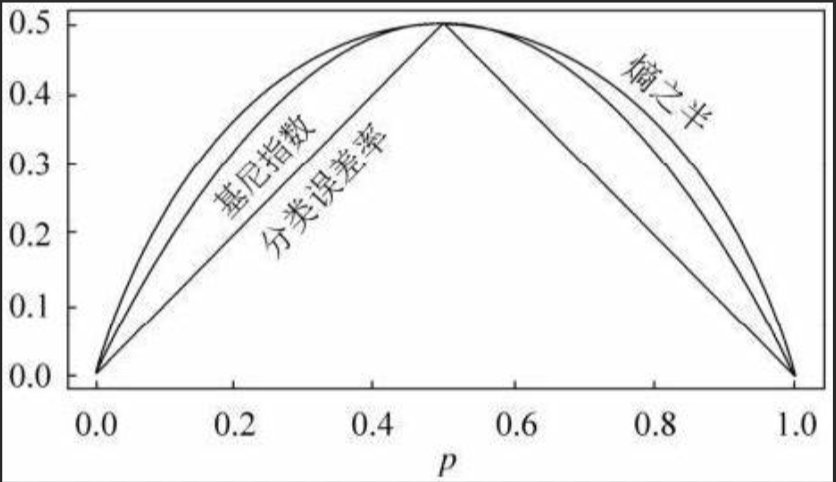
\includegraphics[scale=0.5]{3.png} \end{figure}
\end{solution}

\newpage

\section{[20pts] Training a Decision Tree}
剪枝(pruning)是决策树学习算法对抗“过拟合”的主要手段.考虑下面的训练集:共计8个训练样本,每个训练样本有三个特征属性$X,Y,Z$和标签信息.详细信息如表\ref{problem2_training_set}所示.
\begin{table}[ht]
    \centering
	\setlength{\abovecaptionskip}{0pt}
	\setlength{\belowcaptionskip}{5pt}
    \caption{训练集信息}
	\label{problem2_training_set}
    %\tabcolsep 15pt
    \begin{tabular}{cccc|c||cccc|c}
        \hline 
        编号 & $X$ & $Y$ & $Z$ & $f$ & 编号 & $X$ & $Y$ & $Z$ & $f$ \\
    \hline1 &   1 &  1 &   0 &   1 &   5 &    0 &   0 &   0 &   0\\
          2 &   1 &  1 &   1 &   1 &   6 &    1 &   0 &   1 &   0 \\
          3 &   0 &  0 &   1 &   0 &   7 &    1 &   1 &   0 &   1\\
          4 &   0 &  1 &   0 &   0 &   8 &    0 &   1 &   1 &   1\\
        \hline
    \end{tabular}
\end{table}
\begin{enumerate}
	\item[(1)] \textbf{[5pts]} 请通过训练集中的数据训练决策树,要求使用“信息增益”(information gain)作为划分准则.(需说明详细计算过程)
	\item[(2)] \textbf{[10pts]} 进一步考虑如表\ref{problem2_validation_set}所示的验证集,对上一问得到的决策树基于这一验证集进行预剪枝、后剪枝.生成叶子结点时,若样例最多的类别不唯一,可任选其中一类.请画出所有可能的剪枝结果.(需说明详细计算过程)
	\begin{table}[ht]
		\centering
		\setlength{\abovecaptionskip}{0pt}
		\setlength{\belowcaptionskip}{5pt}
		\caption{验证集信息}
		\label{problem2_validation_set}
		\begin{tabular}{cccc|c}
		\hline
		编号 & $X$ & $Y$ & $Z$ & $f$ \\ \hline
		  9 &   1 &   1&   1&    1\\
		  10 &   1&    0&   1&    0\\
		  11 &   1&    0&   1&    1\\
		  12 &   0&    1&   0&    0\\
		  13 &   0&    1&   1&    1\\
		  14 &   1&    0&   0&    0\\ \hline
		\end{tabular}
	\end{table}
	\item[(3)] \textbf{[5pts]}请给出预剪枝决策树和后剪枝决策树分别在训练集、验证集上的准确率. 结合本题的结果,讨论预剪枝与后剪枝在欠拟合风险、泛化能力以及训练时间开销层面各自的特点. 
\end{enumerate}



\begin{solution}
	此处用于写解答(中英文均可)
	使用sklearn库实现效果如下:
	\begin{figure}[H] \centering  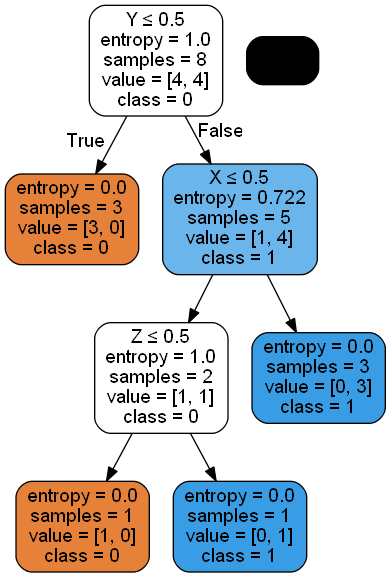
\includegraphics[scale=0.5]{tree.png} \end{figure}
	\begin{enumerate}
		\item[(1)]
		信息熵为 $\text{Ent}(D) = -(\frac{1}{2}\log_2 \frac{1}{2} + \frac{1}{2}\log_{2}\frac{1}{2}) = 1$,首先用属性X划分得到
		\begin{align*}
			\text{Ent}(D^1) &= -\left(\frac{3}{4}\log_2 \frac{3}{4} + \frac{1}{4}\log_2 \frac{1}{4}\right) \approx 0.811 \\
			\text{Ent}(D^2) &= -\left(\frac{1}{4}\log_2 \frac{1}{4} + \frac{3}{4}\log_2 \frac{3}{4}\right) \approx 0.811 \\
			\text{Gain}(D,X) &= 1-\left(\frac{1}{2}\times 0.811 + \frac{1}{2}\times 0.811\right) = 0.189
		\end{align*}
		用属性Y划分可得
		\begin{align*}
			\text{Ent}(D^1) &= -\left(\frac{4}{5}\log_2 \frac{4}{5} + \frac{1}{5}\log_2 \frac{1}{5}\right) \approx 0.722 \\
			\text{Ent}(D^2) &= -(0 + 1\cdot \log_2 1) = 0 \\
			\text{Gain}(D,Y) &= 1-\left( \frac{5}{8} \times 0.722\right) = 0.54875
		\end{align*}
		用属性Z划分可得
		\begin{align*}
			\text{Ent}(D^1) &= -\left( \frac{1}{2} \log_2 \frac{1}{2} + \frac{1}{2}\log_2 \frac{1}{2} \right) = 1 \\
			\text{Ent}(D^2) &= -\left( \frac{1}{2}\log_2 \frac{1}{2} + \frac{1}{2} \log_2 \frac{1}{2} \right) = 1 \\
			\text{Gain}(D,Z) &= 1- (\frac{1}{2}\times 1 + \frac{1}{2} \times 1) = 0
		\end{align*}
		Y划分得到的信息增益最大,$D_1 = \{1,2,4,7,8\},\quad \text{Ent}(D_1)=0.722$.\\ Y=0的时候,所有节点的标签都是0,所以是叶子节点,只需要对Y=1进行划分.
		\\若用属性X进行划分
		\begin{align*}
			\text{Ent}(D^1) &= 0 \\
			\text{Ent}(D^2) &= 1 \\
			\text{Gain}(D_1,X) &= 0.322
		\end{align*}
		\\若根据属性Z划分
		\begin{align*}
			\text{Ent}(D^1) &= 0 \\
			\text{Ent}(D^2) &= -(\frac{2}{3}\log_2\frac{2}{3} + \frac{1}{3}\log_2 \frac{1}{3}) = 0.918 \\
			\text{Gain}(D_1, Z) &= 0.722-0.918\times 0.6 = 0.1712 
		\end{align*}
		因为X的信息增益最大,根据属性X进行划分,X=1时,均分类为1,所以是一个叶子节点,X=0使用Z进行划分,同理,Z=1,Z=0各为一个叶子节点.
		\\最终的决策树如下图所示:
		\begin{figure}[H]
			\centering
			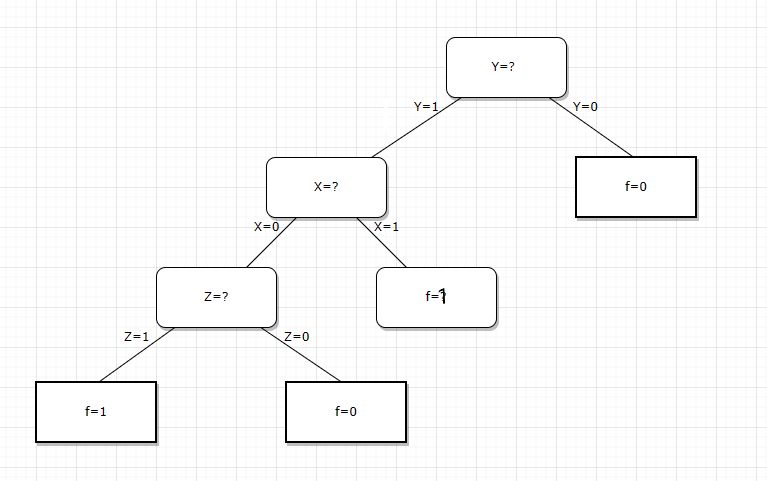
\includegraphics[scale=0.5]{1.png}
			\label{figure}
		\end{figure}		
	
		\item[(2)]
		预剪枝: \\
		属性Y划分前精准度为 50\%,划分后精准度为 67\%,所以应该划分. \\
		属性X划分前精准度为 67\%,划分后精准度为 67\%,所以不应划分. \\
		剪枝结果
		\begin{figure}[H]
			\centering
			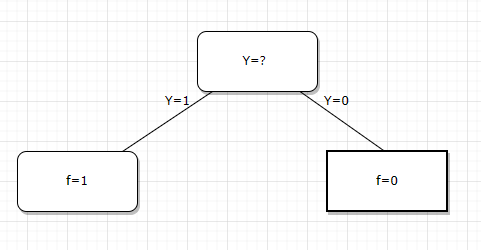
\includegraphics[scale=0.5]{2.png}
			\label{figure}
		\end{figure}
	
		后剪枝:\\	
		该决策树在验证集上的精度为 83\%. \\
		如果不划分 Z,验证集精度为 67 \%,所以不进行剪枝.\\
		如果不划分 X,验证集精度为 83\%,所以可以不进行剪枝.(根据奥卡姆剃刀准则,通常要剪枝,这里与教材一致,并没有剪枝) \\
		如果不划分 Y,验证集精度为 50 \%,所以不进行剪枝. \\
		剪枝结果
		\begin{figure}[H]
			\centering
			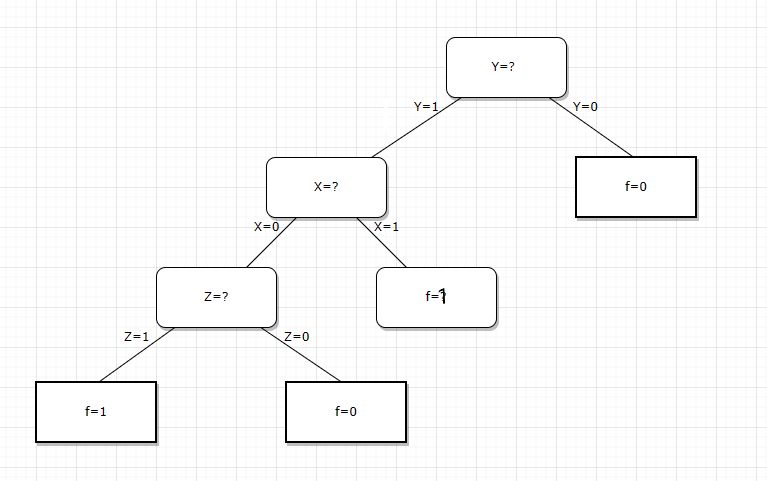
\includegraphics[scale=0.5]{1.png}
			\label{figure}
		\end{figure}
	
		\item[(3)]
		预剪枝决策树训练集精度为87.5\%,验证集精度为66\%. \\
		后剪枝决策树训练集精度为100\%,验证集精度为83\%\\
		预剪枝和后剪枝在欠拟合风险、泛化能力和训练时间开销方面各有不同的特点。

		- 欠拟合风险\\
		预剪枝是在决策树生成的过程中就进行剪枝,可能会在树还没有完全生成时就停止,因此可能会导致欠拟合的问题。而后剪枝则是在树生成完成后再进行剪枝,可以更充分地利用训练集的信息,因此相对来说欠拟合的风险较小。
		
		- 泛化能力\\
		预剪枝通常会限制树的深度、叶子节点数或信息增益的阈值等,因此可能会过早地停止树的生成过程,从而导致模型的泛化能力不足。后剪枝则是在树生成完成后,通过对叶子节点进行合并或修剪,进一步提高模型的泛化能力。
		
		- 训练时间开销\\
		预剪枝是在决策树生成的过程中就进行剪枝,因此训练时间开销较小。而后剪枝则是在树生成完成后再进行剪枝,需要遍历整棵树进行修剪,因此训练时间开销较大。
		
		预剪枝对于小数据集或者数据特征数很多的数据集来说效果较好,因为预剪枝不需要遍历整棵树,训练速度较快,同时也不容易出现过拟合的问题;后剪枝对于大数据集来说效果较好,因为后剪枝可以更充分地利用训练集的信息,提高泛化能力,但是训练时间会比较长。

		
	\end{enumerate}
	~\\
	~\\
	~\\
\end{solution}

\newpage

\section{[20pts] Kernel Function}
核函数是 SVM 中常用的工具,其在机器学习中有着广泛的应用与研究. 请自行阅读学习《机器学习》第 6.3 节, 并回答如下问题.
\begin{enumerate}
	\item[(1)] \textbf{[5pts]} 试判断 $\kappa(\x, \z) = \left(\langle\x, \z\rangle - 1\right)^2$ 是否为核函数,并给出证明或反例.
	\item[(2)] \textbf{[5pts]} 试证明:对于半正定矩阵 $\A$,总存在半正定矩阵 $\C$,成立$\A = \C^\top \C$
	\item[(3)] \textbf{[5pts]} 试证明:若 $\kappa_1$ 和 $\kappa_2$ 为核函数, 则两者的直积
	\[
	\kappa_1 \otimes \kappa_2(\x, \z)=\kappa_1(\x, \z) \kappa_2(\x, \z)
	\]
	也是核函数;
	\item[(4)] \textbf{[5pts]} 试证明 $\kappa(\x, \z) = \langle\x, \z\rangle^p$ 对 $\forall p\in\mathbb{Z}_+(p<\infty)$ 均为核函数.

	
\end{enumerate}

\begin{solution}
	此处用于写解答(中英文均可)
	\begin{enumerate}
		\item[(1)]
		不是核函数. \\
		举反例如下:\\数据集$D=\{\bds{x_1},\bds{x_2}\}=\{(1,0), (0,1)\}$ \\
		则$\kappa(\bds{x_1}, \bds{x_1}) = 0, \kappa(\bds{x_1},\bds{x_2}) = 1, \kappa(\bds{x_2}, \bds{x_1}) = 1, \kappa(\bds{x_2}, \bds{x_2})=0$ \\
		核矩阵:\\
		\begin{equation}
			\left(
			\begin{array}{cc}
				0 & 1 \\
				1 & 0
			\end{array}
			\right)
		\end{equation}
		不是半正定矩阵.
		\item[(2)]
		因为 $\mathbf{A}$ 为半正定矩阵, 设其为 $\mathrm{n}$ 阶矩阵, 其特征值 $\lambda_1, \lambda_2, \ldots, \lambda_n$ 均大于等于 0 , 则存在正 交矩阵 $\mathbf{P}$ 使得
		$$
		\begin{aligned}
		\mathbf{A} & =\mathbf{P} \operatorname{diag}\left\{\lambda_1, \lambda_2, \ldots, \lambda_n\right\} \mathbf{P}^{-1} \\
		& =\mathbf{P} \operatorname{diag}\left\{\sqrt{\lambda}_1, \sqrt{\lambda}_2, \ldots, \sqrt{\lambda}_n\right\} \mathbf{P}^{-1} \mathbf{P} \operatorname{diag}\left\{\sqrt{\lambda}_1, \sqrt{\lambda}_2, \ldots, \sqrt{\lambda}_n\right\} \mathbf{P}^{-1} \\
		& =\mathbf{P} \operatorname{diag}\left\{\sqrt{\lambda}_1, \sqrt{\lambda}_2, \ldots, \sqrt{\lambda}_n\right\} \mathbf{P}^{-1}\left(\mathbf{P}^{-1}\right) \top \operatorname{diag}\left\{\sqrt{\lambda}_1, \sqrt{\lambda}_2, \ldots, \sqrt{\lambda}_n\right\} \mathbf{P}^ \top \\
		& =\mathbf{P} \operatorname{diag}\left\{\sqrt{\lambda}_1, \sqrt{\lambda}_2, \ldots, \sqrt{\lambda}_n\right\} \mathbf{P}^{-1}\left(\mathbf{P} \operatorname{diag}\left\{\sqrt{\lambda}_1, \sqrt{\lambda}_2, \ldots, \sqrt{\lambda}_n\right\} \mathbf{P}^{-1}\right)^ \top
		\end{aligned}
		$$
		由于$\mathbf{A}=\mathbf{C}^{\top} \mathbf{C}$ 成立, 且 $\mathbf{C}$ 为半正定矩阵
		令 $\mathbf{C}=\mathbf{P}\left\{\sqrt{\lambda}_1, \sqrt{\lambda}_2, \ldots, \sqrt{\lambda}_n\right\} \mathbf{P}^{-1}$
		\item[(3)]
		设 $\kappa(\x,\z) = \kappa_1\bigotimes \kappa_2(\x,\z)$,$\kappa_1, \kappa_2$为核函数,则考虑核矩阵的半正定性
		\begin{align*}
			\y^T \mathbf{K} \y &= \y^T \begin{bmatrix}
				\kappa_1(\bds{x}_1, \bds{x}_1)\kappa_2(\bds{x}_1,\bds{x}_1) & \dots & \kappa_1(\bds{x}_1, \bds{x}_m)\kappa_2(\bds{x}_1,\bds{x}_m) \\
				\vdots & \ddots &\vdots \\
				\kappa_1(\bds{x}_m, \bds{x}_1)\kappa_2(\bds{x}_m,\bds{x}_1) & \dots & \kappa_1(\bds{x}_m, \bds{x}_m)\kappa_2(\bds{x}_m,\bds{x}_m)
			\end{bmatrix} \y \\
			&= \sum_{i=1}^{m}\sum_{j=1}^{m} \kappa_1(\bds{x}_i, \bds{x}_j)\kappa_2(\bds{x}_i,\bds{x}_j)\y_i\y_j \\
			&= \text{tr}\left( \begin{bmatrix}
				\y_1\kappa_1(\bds{x}_1, \bds{x}_1) & \dots & \y_1\kappa_1(\bds{x}_1, \bds{x}_m) \\
				\vdots & \ddots & \vdots \\
				\y_m\kappa_1(\bds{x}_m, \bds{x}_1) & \dots & \y_m\kappa_1(\bds{x}_m, \bds{x}_m) 
			\end{bmatrix} \begin{bmatrix}
				\y_1\kappa_2(\bds{x}_1, \bds{x}_1) & \dots & \y_1\kappa_2(\bds{x}_m, \bds{x}_1) \\
				\vdots & \ddots & \vdots \\
				\y_m\kappa_2(\bds{x}_1, \bds{x}_m) & \dots & \y_m\kappa_2(\bds{x}_m, \bds{x}_m)
			\end{bmatrix}  \right) \\
			&= \text{tr} \left( \begin{bmatrix}
				\y_1 & & \\
				& \ddots & \\
				& & \y_m
			\end{bmatrix} \mathbf{K}_1 \begin{bmatrix}
				\y_1 & & \\
				& \ddots & \\
				& & \y_m
			\end{bmatrix} \mathbf{K}_2^T \right) \\
			& \text{由于} \mathbf{K}_1, \mathbf{K}_2 \text{均为半正定矩阵,所以有} \mathbf{K}_1 = \mathbf{C}^T\mathbf{C}, \mathbf{K}_2 = \mathbf{D}^T\mathbf{D} \text{,所以有} \\
			&= \text{tr}\left( \begin{bmatrix}
				\y_1 & & \\
				& \ddots & \\
				& & \y_m
			\end{bmatrix} \mathbf{C}^T\mathbf{C} \begin{bmatrix}
				\y_1 & & \\
				& \ddots & \\
				& & \y_m
			\end{bmatrix} \mathbf{D}^T\mathbf{D} \right) \\
			&\text{由于以上矩阵均为方阵,且交换矩阵乘法顺序不改变矩阵的迹,所以} \\
			&= \text{tr}\left( \left(\mathbf{C}\begin{bmatrix}
				\y_1 & & \\
				& \ddots & \\
				& & \y_m
			\end{bmatrix} \mathbf{D}^T \right)^T \mathbf{C} \begin{bmatrix}
				\y_1 & & \\
				& \ddots & \\
				& & \y_m
			\end{bmatrix} \mathbf{D}^T \right) \\
			&= \text{tr} (\mathbf{Q}^T\mathbf{Q}) \geq 0
		\end{align*}
		所以核矩阵是半正定的,所以 $\kappa(\x,\z) = \kappa_1\bigotimes \kappa_2(\x,\z)$也是核函数.
		\item[(4)]  
		由(3)结论,我们只需要证明$\kappa(x, z) = x^{T}z$是核函数即可\\
		由核函数的定义,假设输入空间为$\mathcal{X}$\\
		定义映射$\phi: \mathcal{X} \rightarrow \mathcal{H}$ ,
		$\phi (x) = x$ \\
		那么对所有的$x,z\in \mathcal{X}$\\
		$\kappa(x, z) = x^{T}z = \phi (x)\cdot\phi (z)$\\
		所以$\kappa$是核函数,进而$\kappa(\x, \z) = \langle\x, \z\rangle^p$ 对 $\forall p\in\mathbb{Z}_+(p<\infty)$ 也为核函数。
	\end{enumerate}
	\end{solution}

	\end{document}
